% !TEX TS-program = pdflatex
% !TEX encoding = UTF-8 Unicode

% This is a simple template for a LaTeX document using the "article" class.
% See "book", "report", "letter" for other types of document.

\documentclass[11pt]{article} % use larger type; default would be 10pt

%\usepackage{etex}

\usepackage[utf8]{inputenc} % set input encoding (not needed with XeLaTeX)
\usepackage[french]{babel}

%%% Examples of Article customizations
% These packages are optional, depending whether you want the features they provide.
% See the LaTeX Companion or other references for full information.

%%% PAGE DIMENSIONS
\usepackage{geometry} % to change the page dimensions
\geometry{a4paper} % or letterpaper (US) or a5paper or....
% \geometry{margin=2in} % for example, change the margins to 2 inches all round
% \geometry{landscape} % set up the page for landscape
%   read geometry.pdf for detailed page layout information

\usepackage{graphicx,float} % support the \includegraphics command and options
\usepackage{caption}
\usepackage{subcaption}
% \usepackage[parfill]{parskip} % Activate to begin paragraphs with an empty line rather than an indent

%%% PACKAGES
\usepackage{booktabs} % for much better looking tables
\usepackage{array} % for better arrays (eg matrices) in maths
\usepackage{paralist} % very flexible & customisable lists (eg. enumerate/itemize, etc.)
\usepackage{verbatim} % adds environment for commenting out blocks of text & for better verbatim
%\usepackage{subfig} % make it possible to include more than one captioned figure/table in a single float
% These packages are all incorporated in the memoir class to one degree or another...

%%% HEADERS & FOOTERS
\usepackage{fancyhdr} % This should be set AFTER setting up the page geometry
\pagestyle{fancy} % options: empty , plain , fancy
\renewcommand{\footrulewidth}{1pt} % customise the layout...
%\lhead{}\chead{}\rhead{}
%\lfoot{}\cfoot{\thepage}\rfoot{}
\setlength{\headheight}{24.08003pt}


%%% SECTION TITLE APPEARANCE
\usepackage[immediate]{silence}
\WarningFilter[temp]{latex}{Command} % silence the warning
\usepackage{sectsty}
\DeactivateWarningFilters[temp] % So nothing unrelated gets silenced
%\allsectionsfont{\mdseries} % (See the fntguide.pdf for font help)
% (This matches ConTeXt defaults)

%%% ToC (table of contents) APPEARANCE
\usepackage[nottoc,notlof,notlot]{tocbibind} % Put the bibliography in the ToC
\usepackage[titles]{tocloft} % Alter the style of the Table of Contents
\renewcommand{\cftsecfont}{\rmfamily\mdseries\upshape}
\renewcommand{\cftsecpagefont}{\rmfamily\mdseries\upshape} % No bold!
\setcounter{lofdepth}{2}

%%%packages ajouté par Stefano Losito
\usepackage[style=phys, backend=biber, %
articletitle=true, biblabel=brackets, %
chaptertitle=false, pageranges=false%
]{biblatex}



\usepackage{amssymb}  
\usepackage[x11names]{xcolor}
\newcommand{\hlc}[2][yellow]{ {\sethlcolor{#1} \hl{#2}} }


\DeclareCaptionFont{lightgray}{\color{lightgray}}
\captionsetup{format=hang,justification={justified},labelfont={color=black,footnotesize},textfont={color=black,footnotesize},list=true}
%\captionsetup[sub]{list=true}

\usepackage{enumitem, soul}
\usepackage{physics,amsmath,amsthm}
\usepackage{mathrsfs}
\usepackage{cancel}
\usepackage{scalerel}
\usepackage{upgreek,bm}
\usepackage{mathtools}
\usepackage[hidelinks]{hyperref}
\usepackage[french]{cleveref}
\usepackage{enumitem}
\usepackage{enotez}
\usepackage{tikz} 
\usepackage{pgfplots}
%\usepackage{gensymb}
\pgfplotsset{compat=1.18}


\usepgflibrary{arrows.meta}

%\usepackage{circuitikz}

%\usepackage{mfirstuc}
%\usepackage{siunitx}
\usepackage[acronym,xindy={codepage=utf8},nomain]{glossaries-extra}

\usepackage{titling}
\usepackage{appendix}
%\usepackage{placeins}
\usepackage{lastpage}
%\usepackage[english]{isodate}
\usepackage[en-GB]{datetime2}
\usepackage[final]{pdfpages}
\usepackage{color}
\usepackage{csquotes}

\usepackage{mathdots}

%\usepackage{suffix}
%\usepackage{acronym}

\usepackage{fourier}
\usepackage{arcs}
\usepackage{tipa}
%\usepackage{mathabx}
%\usepackage{mathtools}  
%\mathtoolsset{showonlyrefs} 

\usepackage{lipsum}


\usepackage{xfp}
\usepackage{standalone}
\usepackage{import}
%\usepackage{txfonts}
%\usepackage{ stmaryrd }
%\usepackage{stix}

%\usepackage[autoplay,loop,final]{animate}

\usepackage{footmisc}
%\usepackage[symbol*]{footmisc}
%\renewcommand{\thefootnote}{\fnsymbol{footnote}}

%\usepackage[scaled]{helvet}
%\renewcommand\familydefault{\sfdefault} 
%\usepackage[T1]{fontenc}
%\usepackage{MnSymbol}

\pdfinclusionerrorlevel=1
\pdfminorversion=7
\pdfsuppresswarningpagegroup=1

\newcommand{\titlee}{\color{red}Titre titre}% Title
\newcommand{\datered}{\today} % date of submission
\newcommand{\dated}{{\DTMsetstyle{ddmmyyyy}\DTMdisplaydate{2023}{5}{15}{0}}} % du dd.mm.aa
\newcommand{\datef}{{\DTMsetstyle{ddmmyyyy}\DTMdisplaydate{2023}{5}{26}{4}}} % au dd.mm.aa 
\newcommand{\auteur}{\color{blue}Auteur} % Auteur 
%\newcommand{\nlabo}{9} % nb Laboratory
\newcommand{\assistant}{\color{dark-green}Assistant} % Name assistant
%\newcommand{\groupe}{S} % Groupe (A-Z)

\newcommand{\tqte}[1]{\textquotedblleft #1 \textquotedblright}

%\renewcommand{\labelitemi}{--}
\newcommand{\ac}[1]{\acrshort{#1}}
%\newcommand{}[]{}



\hypersetup{
	pdfencoding=auto,
	colorlinks=true,
	linkcolor=black,
	filecolor=magenta,
	urlcolor=blue,
	pdfauthor={\auteur},
 	pdftitle={\jobname},
 	pdfkeywords={},
 	pdfsubject={\jobname},
 	pdfcreator={\auteur},
 	pdflang={English}
}

\urlstyle{same}

\pagestyle{fancy}
\fancyhf{}
\fancyfoot{}
\lfoot{\jobname}
\rhead{UniGe, Physique}
\chead{\titlee}
\cfoot{Page \thepage \hspace{1pt} of {
	\hypersetup{linkcolor=black}\hspace{1pt}\pageref{last page}}}
\rfoot{\today}
\lhead{\auteur}

%\bibliographystyle{unsrt}
%%% END Article customizations


%\newacronym{sr}{SR}{special relativity}

%\newglossaryentry{het}
%{
%name={Ettingshausen's effect},
%description={is the resistance due to the heat caused by the accumulation of electrons caused by \gls{he}}
%}

%\makenoidxglossaries

%%% The "real" document content comes below...

\title{\titlee \\ \normalcolor TPI}
\author{\auteur}
\date{\today}

%\date{} % Activate to display a given date or no date (if empty),
% otherwise the current date is printed 

\graphicspath{{imagini/}}
\makeatletter
\def\input@path{{input/}}
\makeatother
\addbibresource{biblio.bib}


\begin{document}


	%\begingroup 

\inputencoding{cp1252}%

\thispagestyle{empty}

\begin{picture}(0,0)
	\put(-95,-763){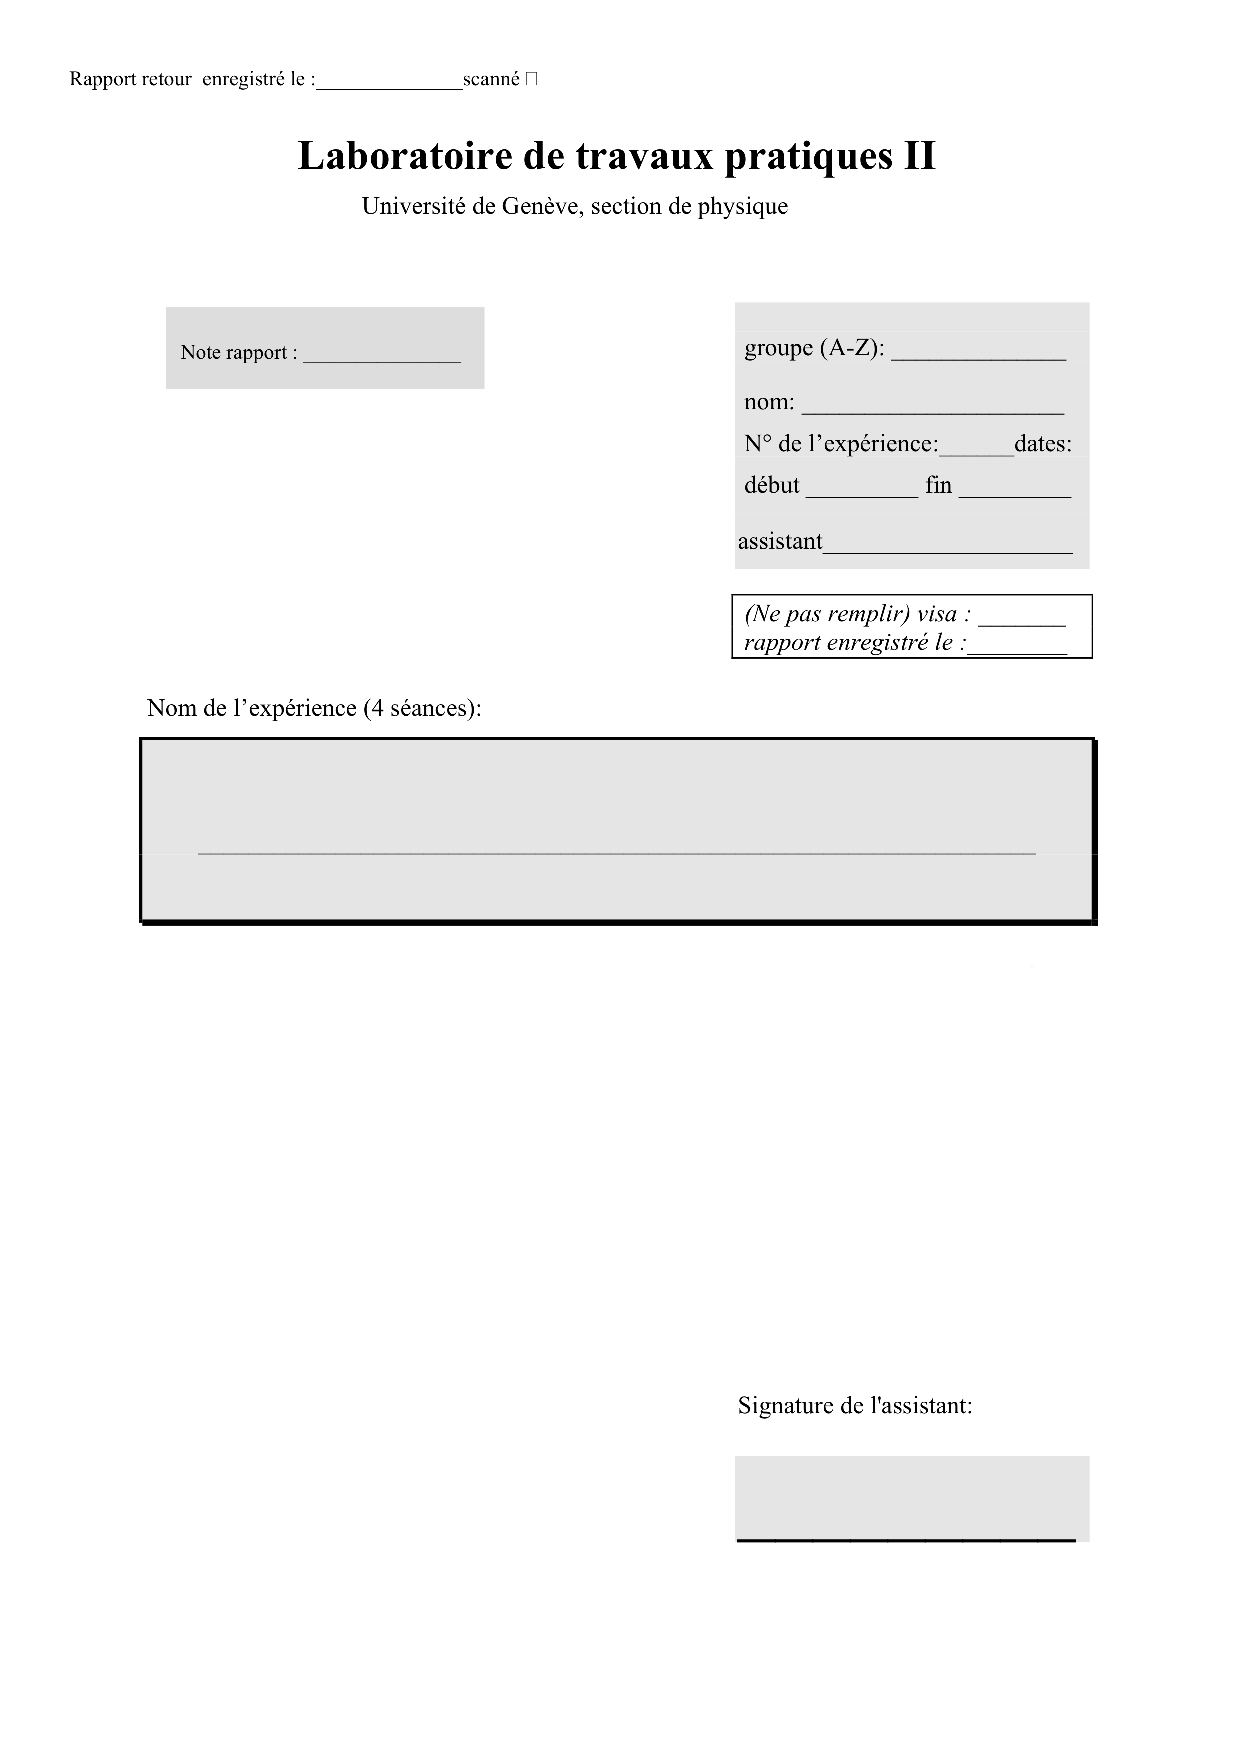
\includegraphics{tete.pdf}}
	 \put(195,-310){\makebox(0.1,0.1){\Huge{\titlee}}}
	 \put(366,-85){\makebox(0.1,0.1){\groupe}}
	 \put(340,-111){\makebox(0.1,0.1){\nome}}
	 \put(370,-132){\makebox(0.1,0.1){\nlabo}}
	 \put(360,-180){\makebox(0.1,0.1){\assistant}}
	 \put(292,-155){\dated}
	 \put(367,-155){\datef}
  \end{picture}

\endgroup
	%\newpage
	\bigskip
	\pretitle{\begin{center}
			
\includegraphics{logo.jpg}\LARGE\\}
		\posttitle{\end{center}}
	
	\maketitle
	
	\pagenumbering{gobble}
	\newpage
	\pagenumbering{arabic}
\tableofcontents

\listoffigures

\pagebreak
\hypersetup{linkcolor=blue}
\section{Introduction}

\lipsum[1]

\subsection{But}

\lipsum[1]
\footnote{\lipsum[1][1]}

\subsection{À propos de \titlee}

\lipsum[1]


\section{Théorie}

\lipsum[1]
\begin{equation}
	E=h\nu
\end{equation}
avec, $E$ l'énergie, h, la constante de Planck, et $\nu$ la fréquence. 
\lipsum[2-3]

\section{Expériences}
\lipsum[1-2]
\begin{figure}[H]
	\centering
	\begin{tikzpicture}[>=stealth]
		\begin{axis}[
			hide axis,
			domain=-1:1,
			samples=10,
			xmin=-1,xmax=1,
			ymin=-1,ymax=1,
			zmin=-1,zmax=1,
			]


			%magnetic field
			\pgfplotsinvokeforeach{-1,-.5,0,.5,1}{
			  \addplot3[cyan,quiver,-stealth,
			  point meta={sqrt((x)^2+(y)^2+(z)^2)},
			  quiver={
				u={0},
				v={0},
				w={1},
				colored,scale arrows=.1}]
			  (x,y,#1);
			}

			%receiver
			\draw[fill=gray] (-1,0,0) -- (-0.3,0,0) -- (-0.3,0,0.3)--(-1,0,0.3)--(-1,0,0) ;
			\draw[fill=gray!50] (-1,0.1,0.3) -- (-0.3,0.1,0.3) -- (-0.3,0,0.3)--(-1,0,0.3)--(-1,0.1,0.3) ;
			\draw[fill=gray!30] (-0.3,0,0) -- (-0.3,0,0.3) --(-0.3,0.1,0.3) --(-0.3,0.1,0)-- (-0.3,0,0);
			\draw[fill=blue,rounded corners=1] (-0.65,0,0.10) -- (-0.35,0,0.10) -- (-0.35,0,0.20)--(-0.65,0,0.20)--(-0.65,0,0.10);
		
			
			%radioactive source hole
			\draw[fill=gray] (.6,0,0) -- (0.3,0,0) -- (0.3,0,0.3)--(.6,0,0.3)--(.6,0,0) ;
			\draw[fill=gray!50] (.6,0.3,0.3) -- (0.3,0.3,0.3) -- (0.3,0,0.3)--(.6,0,0.3)--(.6,0.3,0.3) ;
			\draw[fill=gray!30] (0.6,0,0) -- (0.6,0,0.3) -- (0.6,0.3,0.3) -- (0.6,0.3,0) -- (0.6,0,0);
			\draw[fill=gray!150,rounded corners=1] (0.55,0,0.10) -- (0.35,0,0.10) -- (0.35,0,0.20) -- (0.55,0,0.20) -- (0.55,0,0.10);

			%radioactive source
			\draw[fill=red!40!green!60] (0.4,0,0.1)--(0.4,0,0.2)--(0.5,0,0.2)--(0.5,0,0.1)--(0.4,0,0.1);

			%paths
			\draw[thick] (0.45,0,0.2) arc (180:0:-0.42);
			\draw[thick,->] (0.45,0,0.2) arc (180:90:-0.42);
			\draw[thin,-{Circle[cyan]},opacity=0.5] (0.45,0,0.2) arc (180:160:-0.42);

			\draw[thick] (0.45,0,0.15) arc (180:0:-0.48);
			\draw[thick,->] (0.45,0,0.15) arc (180:90:-0.48);
			\draw[thin,-{Circle[cyan]},opacity=0.5] (0.45,0,0.15) arc (180:100:-0.48);

			\draw[thick] (0.45,0,0.1) arc (180:0:-0.52);
			\draw[thick,->] (0.45,0,0.1) arc (180:90:-0.52);
			\draw[thin,-{Circle[cyan]},opacity=0.5] (0.45,0,0.1) arc (180:60:-0.52);


		\end{axis}
	\end{tikzpicture}	
	\caption{Image pour expliquer}
	\label{fig lay : sr}
\end{figure}

\lipsum[2][1] \Cref{fig lay : sr}.

\begin{enumerate}
	\item Une liste 
	\item pour expliquer
	\item comment faire.
\end{enumerate}


\lipsum[1-3]



\section{Discussions}
\lipsum[4][1-3]

\begin{itemize}
	\item Une liste 
	\item pour expliquer
	\item ce qui doit 
	\item être compris.
\end{itemize}


\subsection*{Résultats Notables}

\lipsum[1][1]

\nocite{*}

%\listoftables
%\printendnotes
\printbibliography[heading=bibintoc]
%\printnoidxglossaries

\label{last page}



%\pagebreak
%\newpage
%
%%\rfoot{}
%\cfoot{\thepage/\pageref{LastPage}}
%%\lfoot{}
%\pagenumbering{roman}
%
%\begin{appendices}
%\end{appendices}

\end{document}